% Tela 3 · Minhas reservas (H03 · H04 · H06)
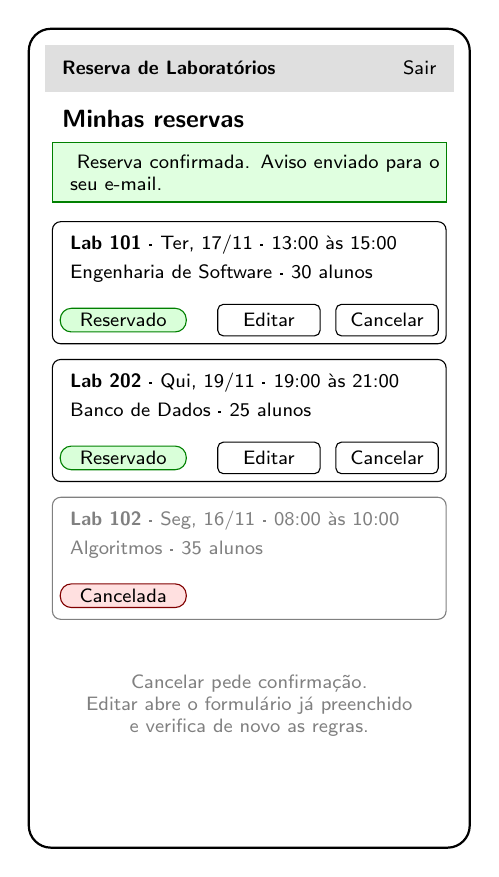
\begin{tikzpicture}[font=\sffamily\scriptsize]
  % aparelho e barra superior
  \draw[thick, rounded corners=8pt] (0,0) rectangle (5.6,10.4);
  \fill[gray!25] (0.2,9.6) rectangle (5.4,10.2);
  \node[anchor=west] at (0.3,9.9) {\textbf{Reserva de Laboratórios}};
  \node[anchor=east] at (5.3,9.9) {Sair};
  \node[anchor=west] at (0.3,9.25) {\small\textbf{Minhas reservas}};

  % aviso de confirmação
  \draw[fill=green!12, draw=green!50!black] (0.3,8.2) rectangle (5.3,8.95);
  \node[anchor=west, text width=4.8cm] at (0.4,8.57) {$\checkmark$ Reserva confirmada. Aviso enviado para o seu e-mail.};

  % reserva 1
  \draw[rounded corners=3pt] (0.3,6.4) rectangle (5.3,7.95);
  \node[anchor=north west] at (0.4,7.9) {\textbf{Lab 101} · Ter, 17/11 · 13:00 às 15:00};
  \node[anchor=north west] at (0.4,7.52) {Engenharia de Software · 30 alunos};
  \draw[fill=green!15, draw=green!50!black, rounded corners=4pt] (0.4,6.55) rectangle (2.0,6.85);
  \node at (1.2,6.7) {Reservado};
  \draw[rounded corners=2pt] (2.4,6.5) rectangle (3.7,6.9); \node at (3.05,6.7) {Editar};
  \draw[rounded corners=2pt] (3.9,6.5) rectangle (5.2,6.9); \node at (4.55,6.7) {Cancelar};

  % reserva 2
  \draw[rounded corners=3pt] (0.3,4.65) rectangle (5.3,6.2);
  \node[anchor=north west] at (0.4,6.15) {\textbf{Lab 202} · Qui, 19/11 · 19:00 às 21:00};
  \node[anchor=north west] at (0.4,5.77) {Banco de Dados · 25 alunos};
  \draw[fill=green!15, draw=green!50!black, rounded corners=4pt] (0.4,4.8) rectangle (2.0,5.1);
  \node at (1.2,4.95) {Reservado};
  \draw[rounded corners=2pt] (2.4,4.75) rectangle (3.7,5.15); \node at (3.05,4.95) {Editar};
  \draw[rounded corners=2pt] (3.9,4.75) rectangle (5.2,5.15); \node at (4.55,4.95) {Cancelar};

  % reserva cancelada
  \draw[rounded corners=3pt, draw=gray] (0.3,2.9) rectangle (5.3,4.45);
  \node[anchor=north west, gray] at (0.4,4.4) {\textbf{Lab 102} · Seg, 16/11 · 08:00 às 10:00};
  \node[anchor=north west, gray] at (0.4,4.02) {Algoritmos · 35 alunos};
  \draw[fill=red!12, draw=red!50!black, rounded corners=4pt] (0.4,3.05) rectangle (2.0,3.35);
  \node at (1.2,3.2) {Cancelada};

  \node[text width=5cm, align=center, gray] at (2.8,1.8) {Cancelar pede confirmação.\\Editar abre o formulário já preenchido\\e verifica de novo as regras.};
\end{tikzpicture}
